\begin{refsection}

\chapter{Detrital geochronology}\label{ch:detrital-R}

Detrital data are arranged in columns that may have unequal lengths:\\

\noindent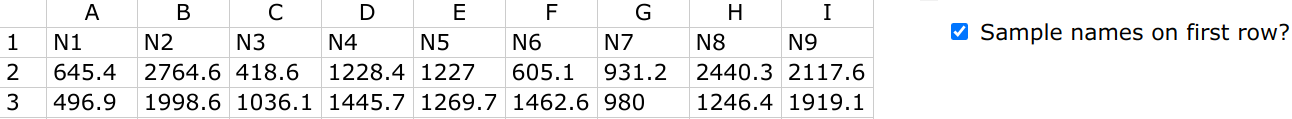
\includegraphics[width=\linewidth]{../figures/detritalInputTable.png}\\

If the `Sample names on first row?' box in the Options menu is
unticked, then the samples will be referred to by their column label
(`A', `B', ...):\\

\noindent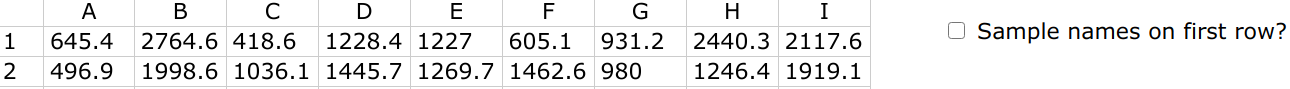
\includegraphics[width=\linewidth]{../figures/detritalInputTableWithoutNames.png}\\

From the CLI, there is no difference between data tables with or
without sample names: \texttt{IsoplotR} automatically detects whether
the first row of the input table contains text or numbers:

\begin{console}
DZ <- read.data('DZ.csv',method='detritals')
\end{console}

This returns a list of named vectors, containing the detrital ages in
each sample. Instead of a column labelled `\texttt{(C)}',
\texttt{IsoplotR}'s GUI uses a text box to report the samples that are
to be omitted from subsequent analysis:

\noindent\begin{minipage}[t]{.4\linewidth}
\strut\vspace*{-\baselineskip}\newline

\includegraphics[width=\linewidth]{../figures/detritalOmit.png}
\end{minipage}
\begin{minipage}[t]{.6\linewidth}
This text box contains a comma-separated list of sample names or
column numbers to omit.
\end{minipage}

\begin{console}
kde(DZ,hide=c('T8','T13'))
\end{console}

\section{Kernel density estimates}

\begin{enumerate}
  
\item The axis limits of the KDEs are the same for all samples to
  facilitate their intercomparison, and their default values are
  chosen so as to cover all the ages in the dataset.

  \noindent\begin{minipage}[t]{.4\linewidth}
\strut\vspace*{-\baselineskip}\newline
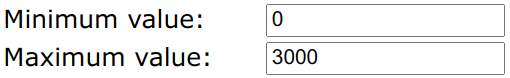
\includegraphics[width=\linewidth]{../figures/detritalKDElimits.png}
\end{minipage}
\begin{minipage}[t]{.6\linewidth}
However, these values can be changed to any other values.
\end{minipage}

\begin{console}
kde(DZ,from=0,to=3000)
\end{console}

\item The inherent positivity of geologic time often results in skewed
  error distributions, which are incompatible with the symmetric
  Gaussian kernel. This skewness can be removed by plotting the KDE on
  a logarithmic scale.

  \noindent\begin{minipage}[t]{.4\linewidth}
\strut\vspace*{-\baselineskip}\newline
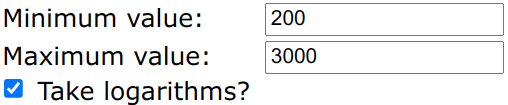
\includegraphics[width=\linewidth]{../figures/detritalKDElogscale.png}
\end{minipage}
\begin{minipage}[t]{.6\linewidth}
  When using a logarithmic transformation, the limits of the time axis
  must consist of strictly positive values.
\end{minipage}

\begin{console}
kde(DZ,log=TRUE,from=200,to=3000)
\end{console}

\item The default kernel bandwidth is computed using the
  \citet{botev2010} algorithm, and generally varies between the
  different samples in the detrital dataset. To facilitate the
  graphical comporison of the distributions, it is useful to apply a
  common kernel bandwidth to all the samples.

\noindent\begin{minipage}[t]{.35\linewidth}
\strut\vspace*{-\baselineskip}\newline

\includegraphics[width=\linewidth]{../figures/detritalKDEsamebandwidth.png}
\end{minipage}
\begin{minipage}[t]{.65\linewidth}
  Ticking the box applies the median value of all the
  \citet{botev2010} bandwidths to all the samples.
\end{minipage}

\begin{console}
kde(DZ,samebandwidth=TRUE)
\end{console}

\item The \citet{botev2010} bandwidth can be replaced by any custom
  value.  Be careful not to over-interpret the KDEs when using a
  bandwidth that is much smaller than the default value!

\noindent\begin{minipage}[t]{.4\linewidth}
  \strut\vspace*{-\baselineskip}\newline
  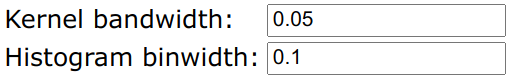
\includegraphics[width=\linewidth]{../figures/detritalKDEcustombandwidth.png}
\end{minipage}
\begin{minipage}[t]{.6\linewidth}
  When the KDE is plotted on a logarithmic scale, the kernel bandwidth
  and histogram bin width are not expressed in Myr but as fractions.
\end{minipage}

Assigning a 5\% bandwidth and 10\% bin width to all the samples:

\begin{console}
kde(DZ,log=TRUE,bw=0.05,binwidth=0.1)
\end{console}

\item\noindent\begin{minipage}[t]{.18\linewidth}
\strut\vspace*{-\baselineskip}\newline

\includegraphics[width=\linewidth]{../figures/detritalrug.png}
\end{minipage}
\begin{minipage}[t]{.82\linewidth}
  Rug plots are turned off by default to remove clutter but can be
  turned on by ticking the box.
\end{minipage}

\begin{console}
kde(DZ,rug=TRUE)
\end{console}

\item To facilitate the comparison of the different samples in a
  detrital dataset, it is useful to scale the y-axis of the KDEs so as
  to normalise the area under them to the same value.

\noindent\begin{minipage}[t]{.38\linewidth}
\strut\vspace*{-\baselineskip}\newline

\includegraphics[width=\linewidth]{../figures/detritalKDEnormalise.png}
\end{minipage}
\begin{minipage}[t]{.62\linewidth}
Switching off this option expands the y-axis to its maximum allowable
extent.
\end{minipage}

\begin{console}
kde(DZ,normalise=FALSE)
\end{console}

\item The KDE can be adjusted using \citet{abramson1982}'s square root
  modifier in order to produce an adaptive density estimate.

\noindent\begin{minipage}[t]{.2\linewidth}
\strut\vspace*{-\baselineskip}\newline

\includegraphics[width=\linewidth]{../figures/detritalKDEadaptive.png}
\end{minipage}
\begin{minipage}[t]{.8\linewidth}
Unticking the box uses a fixed bandwidth along the entire time scale.
\end{minipage}

\begin{console}
kde(DZ,adaptive=TRUE)
\end{console}

\end{enumerate}

\section{Cumulative age distributions}

In contrast with the KDE plot, in which each sample is shown in its
own panel, the CADs of multiple samples can be combined in a single
panel. The \texttt{cad()} function works just like the generic version
(Section~\ref{sec:OtherCAD}), apart from its ability to assign a
different colour to each sample, using a colour ramp function such as
\texttt{cm.colors}, \texttt{topo.colors}, \texttt{terrain.colors}, or
\texttt{heat.colors}:\\

\noindent\begin{minipage}[t]{.32\linewidth}
\strut\vspace*{-\baselineskip}\newline

\includegraphics[width=\linewidth]{../figures/detritalCADcol.png}
\end{minipage}
\begin{minipage}[t]{.68\linewidth}
  Each sample in the dataset can be assigned a different colour
  according to one of the palettes that are available from the
  pull-down menu.
\end{minipage}

\begin{console}
cad(DZ,col='topo.colors')
\end{console}

\section{Multidimensional scaling}

\begin{enumerate}

\item By default \texttt{IsoplotR} uses nonmetric MDS to fit the data,
  but this can be changed to classical MDS (Section~\ref{sec:MDS}).
  
  \noindent\begin{minipage}[t]{.18\linewidth}
\strut\vspace*{-\baselineskip}\newline

\includegraphics[width=\linewidth]{../figures/detritalMDSclassical.png}
\end{minipage}
\begin{minipage}[t]{.82\linewidth}
Classical MDS is useful when the nonmetric MDS configuration collapses
into a point, which can happen for small datasets ($< 10$~samples,
say).
\end{minipage}

\begin{console}
mds(DZ,classical=TRUE)
\end{console}

\item\noindent\begin{minipage}[t]{.18\linewidth}
\strut\vspace*{-\baselineskip}\newline
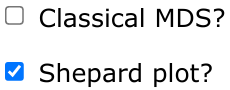
\includegraphics[width=\linewidth]{../figures/detritalMDSshepard.png}
\end{minipage}
\begin{minipage}[t]{.82\linewidth}
The goodness-of-fit of a nonmetric MDS can be visually assessed using
a Shepard plot (Figure~\ref{fig:Shepard}).
\end{minipage}

\begin{console}
mds(DZ,classical=FALSE,shepard=TRUE)
\end{console}

\item It can be useful to augment the MDS configuration with a set of
  nearest neighbour lines (Figure~\ref{fig:DZmds_nnlines}). These
  lines may help assess the success of the ordination, and its ability
  to pull the samples apart into distinct clusters.
  
\noindent\begin{minipage}[t]{.32\linewidth}
\strut\vspace*{-\baselineskip}\newline

\includegraphics[width=\linewidth]{../figures/detritalMDSnnlines.png}
\end{minipage}
\begin{minipage}[t]{.68\linewidth}
  However, the nearest neighbour lines may also clutter the
  configuration to a point where it is better to remove them.
\end{minipage}

\begin{console}
mds(DZ,nnlines=TRUE)
\end{console}

\item\noindent\begin{minipage}[t]{.5\linewidth}
\strut\vspace*{-\baselineskip}\newline
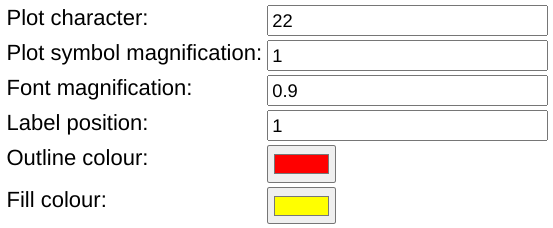
\includegraphics[width=\linewidth]{../figures/detritalMDSotheroptions.png}
\end{minipage}
\begin{minipage}[t]{.5\linewidth}
  The samples can be marked by different plot characters (22 stands
  for a filled square), with sample labels placed either at
  (\texttt{pos=0}), below (\texttt{pos=1}), to the left of
  (\texttt{pos=2}), above (\texttt{pos=3}) or to the right of
  (\texttt{pos=4}) the plot character. The plot characters can be
  scaled separately from the rest of the figure.
\end{minipage}

\begin{console}
mds(DZ,pch=22,cex=0.9,pos=1,bg='yellow',col='red')
\end{console}

\end{enumerate}

\printbibliography[heading=subbibliography]

\end{refsection}
